\section{Desenvolvimento e Resultados}

Nesta seção, são apresentados os resultados obtidos para cada técnica de otimização aplicada, assim como os resultados do algoritmo sem otimização. A análise considera diferentes configurações de simulações, avaliando o impacto de cada técnica no desempenho computacional e na eficiência do modelo.

Para cada técnica, foi conduzida uma série de simulações utilizando combinações variadas de tamanhos de matriz e quantidades de iterações, conforme descrito a seguir:

\begin{itemize}
    \item \textbf{Tamanho da Matriz:} 400, 800, 1200, 1600, 2000
    \item \textbf{Quantidade de Iterações:} 200, 400, 600, 800, 1000
\end{itemize}

Essas combinações foram escolhidas para simular diferentes cenários de complexidade computacional, permitindo uma análise detalhada do desempenho de cada técnica em condições variadas. Os resultados focam nas métricas de tempo de execução.

\subsection{Execução do Algoritmo Compilado com a Flag -O3}
\subsubsection{Configuração do Ambiente de Execução}
\begin{itemize}
    \item Máquina: Notebook IdeaPad Lenovo
    \item CPU: Ryzen 5 5600G
    \item Memória RAM: 12 GB
    \item Compilador: GCC
\end{itemize}

\subsubsection{Resultados}

\begin{figure}[H]
    \centering
    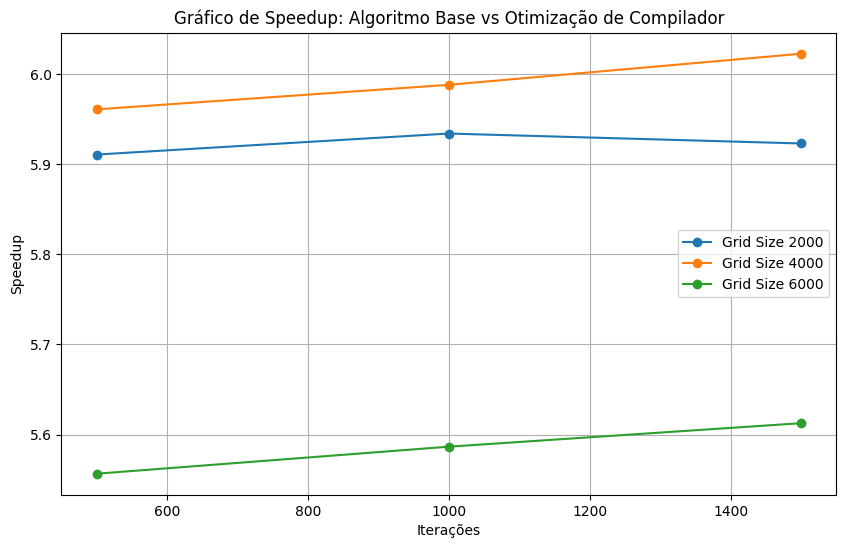
\includegraphics[width=1\linewidth]{./image.png}
    \label{fig:Runtimexblock}
\end{figure}


\subsection{Execução do Algoritmo Paralelizado com OpenMP}
\subsubsection{Configuração do Ambiente de Execução}
\begin{itemize}
    \item Máquina: Notebook IdeaPad Lenovo
    \item CPU: Ryzen 5 5600G
    \item Memória RAM: 12 GB
    \item Compilador: GCC
\end{itemize}

\begin{figure}[H]
    \centering
    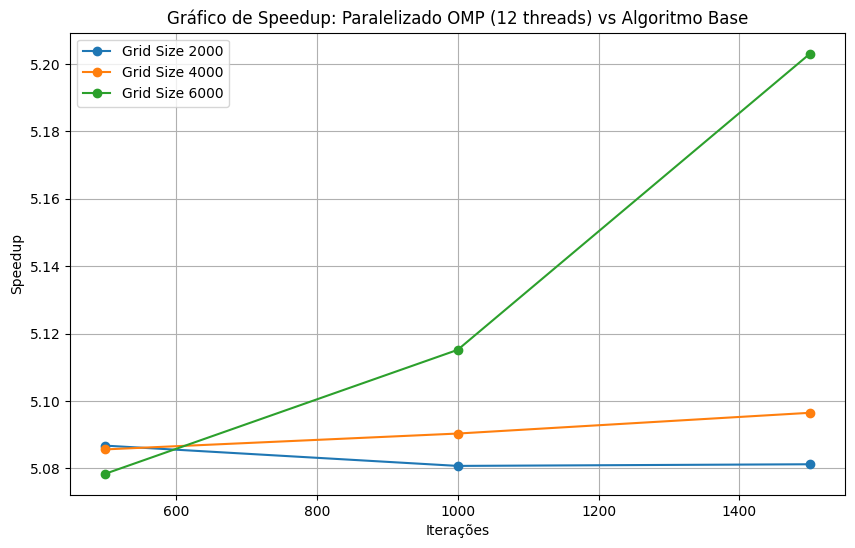
\includegraphics[width=1\linewidth]{./image copy.png}
    \label{fig:Runtimexblock}
\end{figure}

\begin{figure}[H]
    \centering
    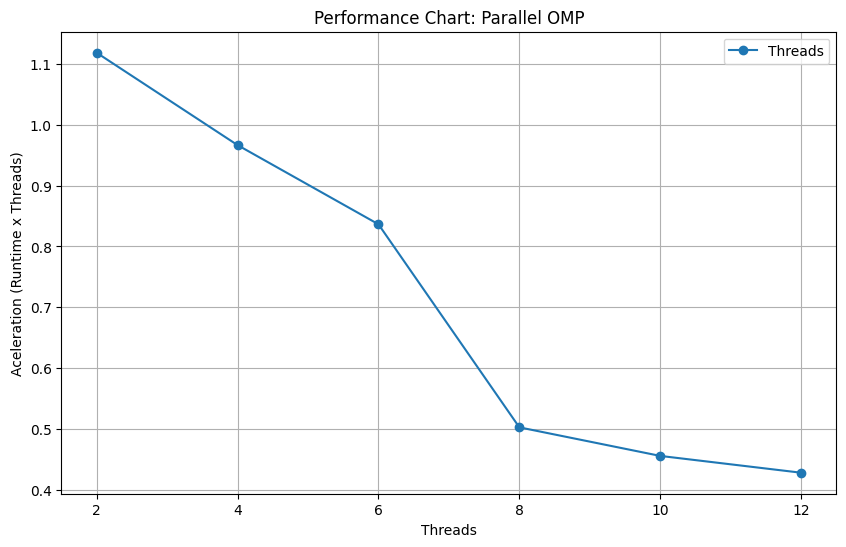
\includegraphics[width=1\linewidth]{./image copy 3.png}
    \label{fig:Runtimexblock}
\end{figure}

\subsection{Execução do Algoritmo Paralelizado com OpenMPI}
\subsubsection{Configuração do Ambiente de Execução}
\begin{itemize}
    \item Máquina: Notebook IdeaPad Lenovo
    \item CPU: Ryzen 5 5600G
    \item Memória RAM: 12 GB
    \item Compilador: GCC
\end{itemize}

\begin{figure}[H]
    \centering
    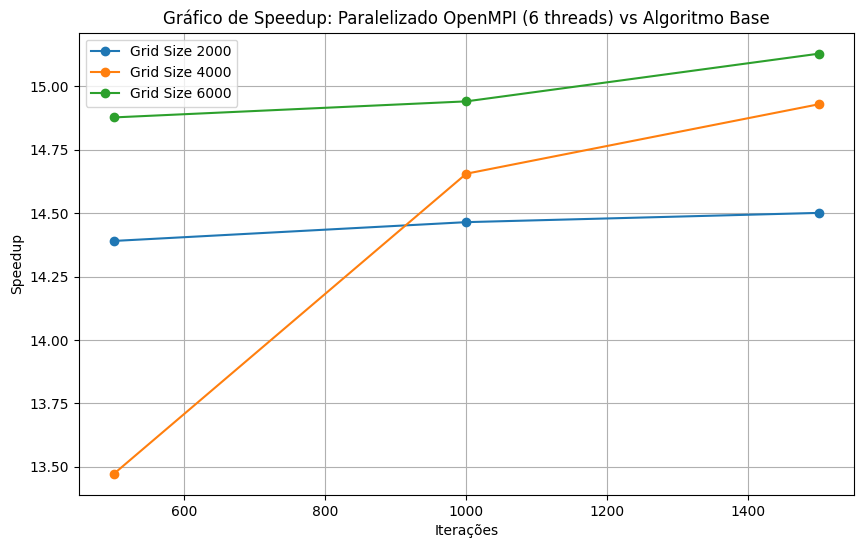
\includegraphics[width=1\linewidth]{./image copy 2.png}
    \label{fig:Runtimexblock}
\end{figure}

\begin{figure}[H]
    \centering
    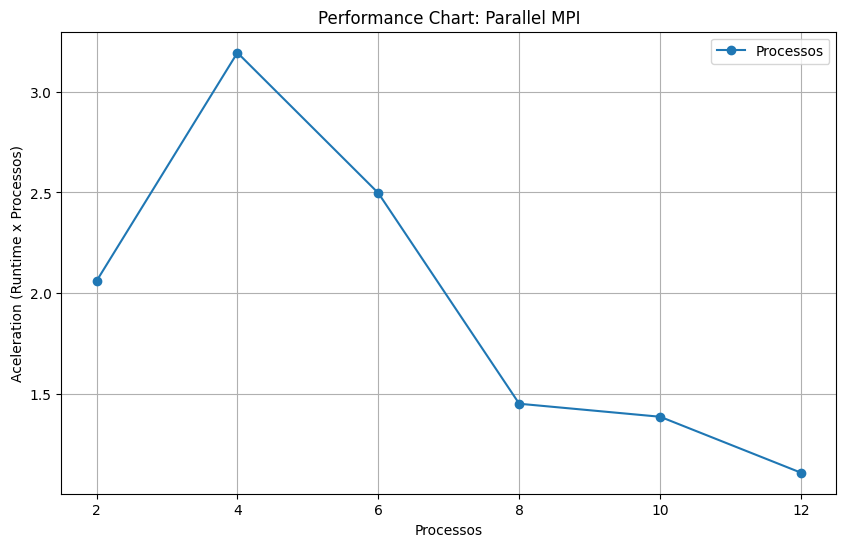
\includegraphics[width=1\linewidth]{./image copy 4.png}
    \label{fig:Runtimexblock}
\end{figure}

\subsection{Execução do Algoritmo Adaptado para CUDA}
\subsubsection{Configuração do Ambiente de Execução}
\begin{itemize}
    \item Máquina: Ambiente Virtual do Google Colab
    \item CPU:
    \item Memória RAM: 16 GB
    \item GPU: T4
    \item Compilador: NVCC (NVIDIA CUDA Compiler)
\end{itemize}

\begin{figure}[H]
    \centering
    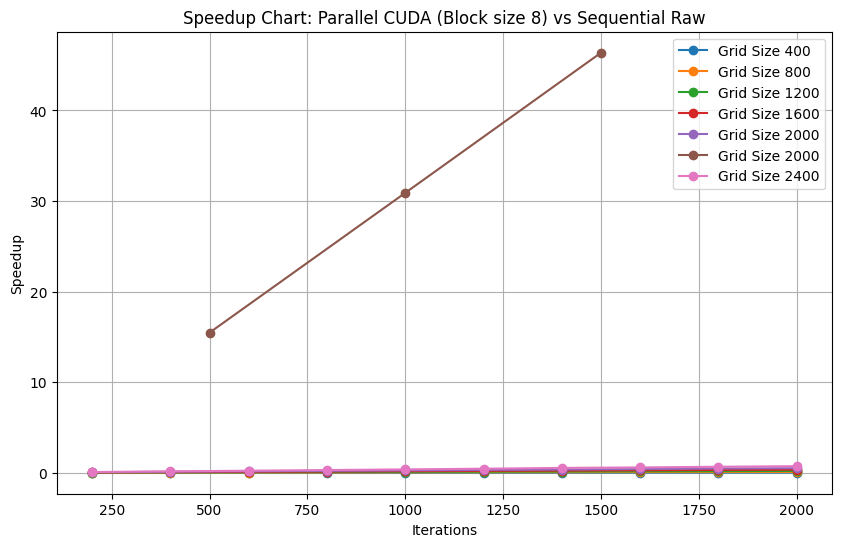
\includegraphics[width=1\linewidth]{./image copy 5.png}
    \label{fig:Runtimexblock}
\end{figure}

\begin{figure}[H]
    \centering
    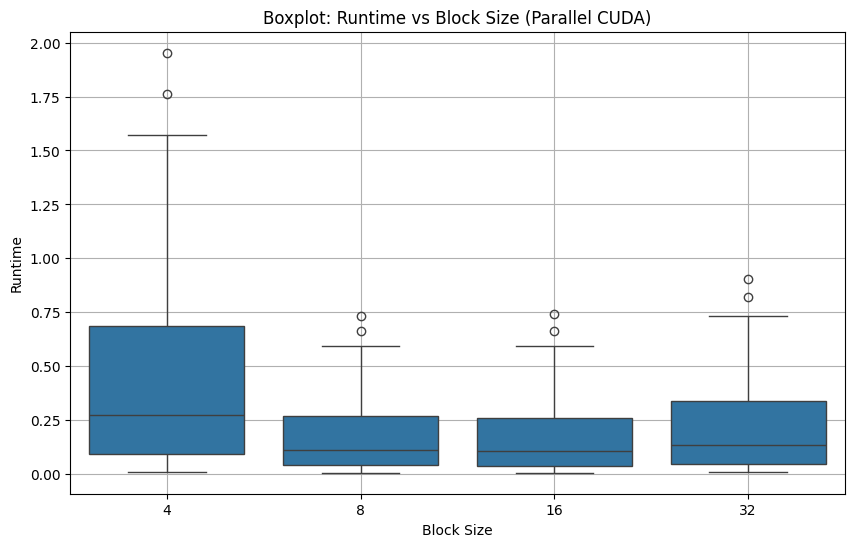
\includegraphics[width=1\linewidth]{./image copy 6.png}
    \label{fig:Runtimexblock}
\end{figure}

\subsection{Comparativo com todos os Métodos}

\begin{figure}[H]
    \centering
    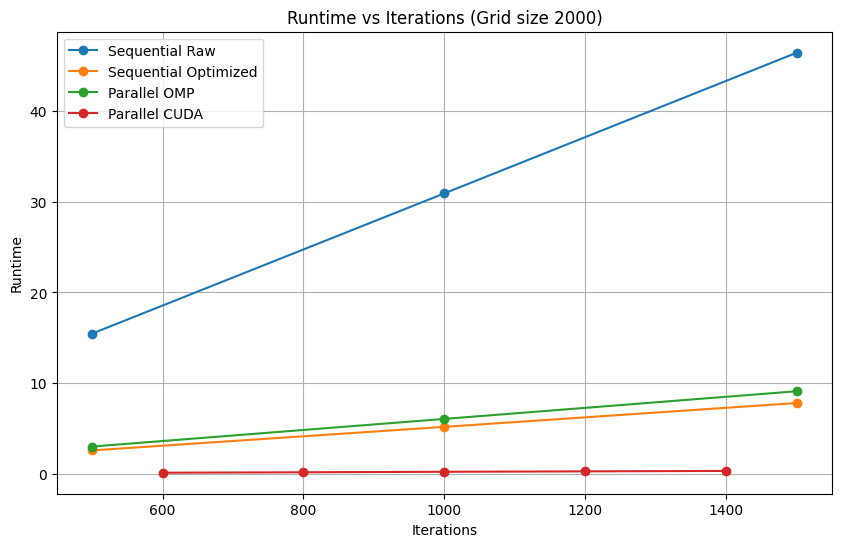
\includegraphics[width=1\linewidth]{./image copy 7.png}
    \label{fig:Runtimexblock}
\end{figure}

\begin{figure}[H]
    \centering
    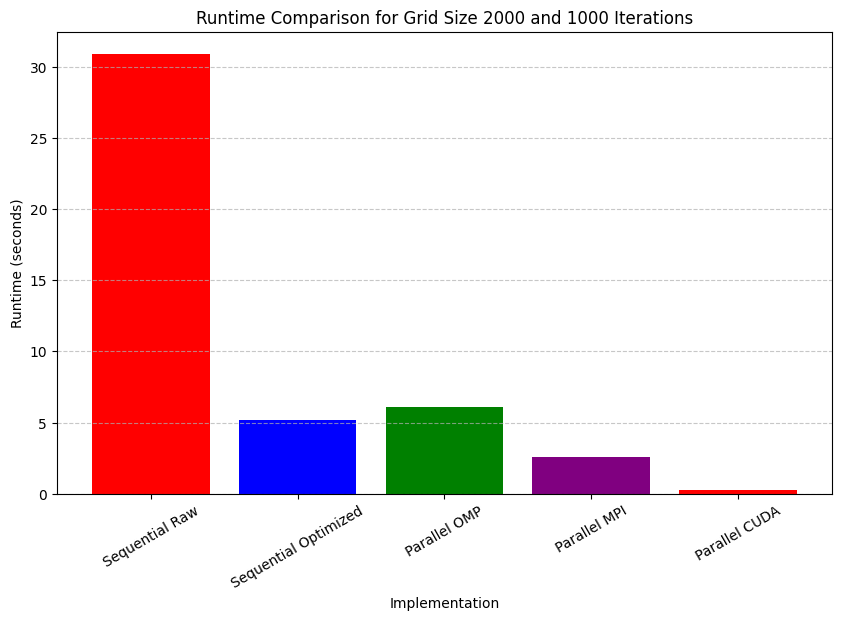
\includegraphics[width=1\linewidth]{./image copy 9.png}
    \label{fig:Runtimexblock}
\end{figure}
